\section*{Supplementary Note S3: Evaluation Detail Retained After Compression}

This note preserves result and protocol detail compressed from the main manuscript without changing the evaluated cases, algorithms, or metrics.

\subsection*{S3.1 Paired observation effects}

The O0--O1 factorial retained all 4608 rows and used 10,000 paired bootstrap resamples. With the E1 RLS kernel unchanged, the paired improvements were 6.6639 percentage points for capacitance MAPE (95\% interval 6.4732--6.8580), 0.97369 percentage points for ESR MAPE (0.92352--1.0265), and 652.20 internal cycles (620.61--683.75). Negative effects from other estimator/metric pairs were retained.

\subsection*{S3.2 Tracking definitions}

The condition thresholds are $C/C_0=0.95/0.90/0.85$ and $r_C/r_0=1.25/1.50/1.75$. A crossing requires two consecutive samples; misses are assigned infinite delay and remain in the records. Threshold delay was not used to choose the primary estimator. Combined nRMSE is the unweighted arithmetic mean of finite C and ESR nRMSE values. Normalized lag uses the largest absolute finite delay among the zero-mean normalized cross-correlation lags and 50\%-trajectory crossings, divided by trajectory duration.

\subsection*{S3.3 Operating-transient traces}

Load, input-voltage, and duty transitions hold physical health constant and measure false-health response. Across the four native-report scenarios, mean peak false capacitance change was 1.3017\% for \TSRLS{} and 0.7570\% for \TSKF{}; mean peak false ESR change was 1.8474\% and 5.1919\%, respectively. \TSRLS{} recovered faster in the evaluated cases.

\begin{figure}[h]
\centering
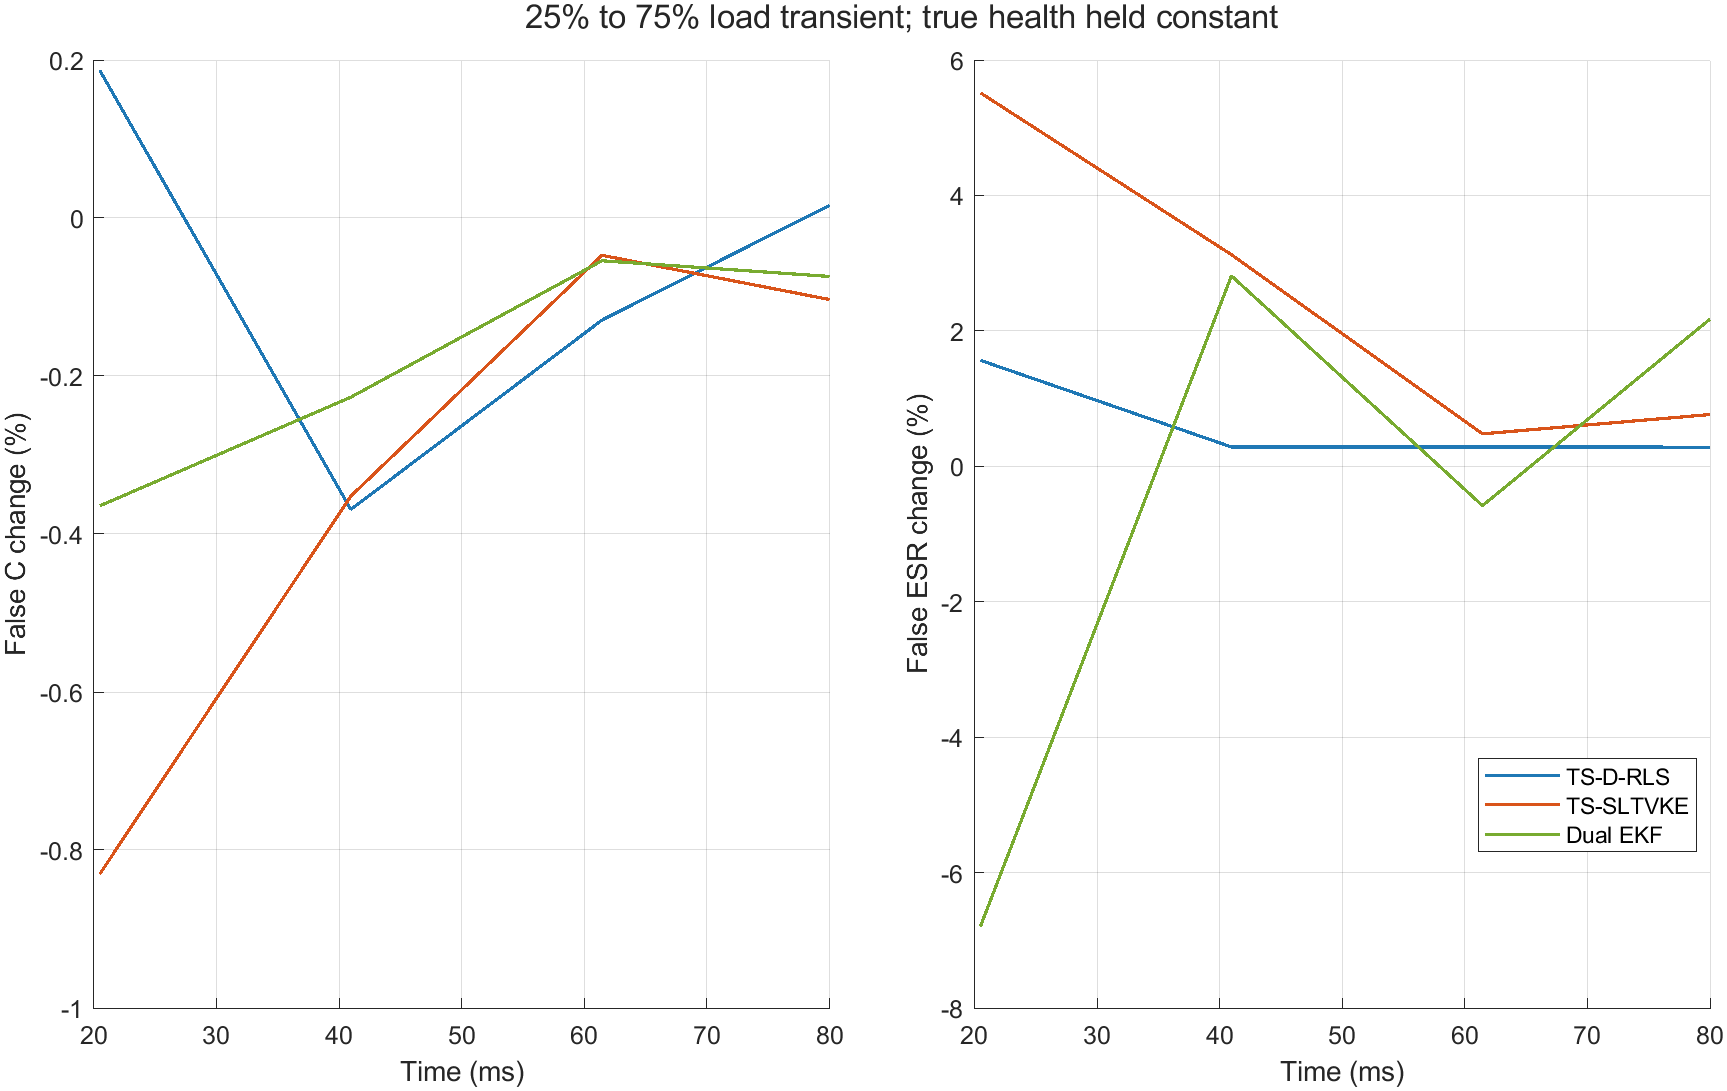
\includegraphics[width=0.95\linewidth]{../figures/fig_operating_transient.png}
\caption*{Fig. S4. False-health response for the load-transient cases with physical health held constant.}
\end{figure}
